\subsection{Results and Discussion}
\label{sec_results_discussion}


\subsubsection{\textbf{Trajectory Estimation Performance}}
Table~\ref{tbl_eval} summarizes the ATE results. \textit{ivS-Graphs} reduces mean ATE by 25.23\% over \textit{vS-Graphs} (second-best), with improvements in 10 of 11 sequences. Improvement scales with trajectory length: sequences exceeding $50\,\text{m}$ (e.g.\ \textit{office1-1}) show average improvement of 30.54\%, while shorter sequences show 18.85\%, confirming that BIM constraints primarily combat drift accumulation in extended operation. This drift-bounding effect is visible in Fig.~\ref{fig:accumulated_drift}: the baseline error grows linearly to $0.8\,\text{m}$, while \textit{ivS-Graphs} stays below $0.2\,\text{m}$ through continuous wall-matching constraints. The single degraded sequence (\textit{office1-4}, -33.33\%) is also one of the shortest ($37.69\,\text{m}$), where minimal drift gives BIM constraints little to correct.


\begin{figure}[t]
    \centering
    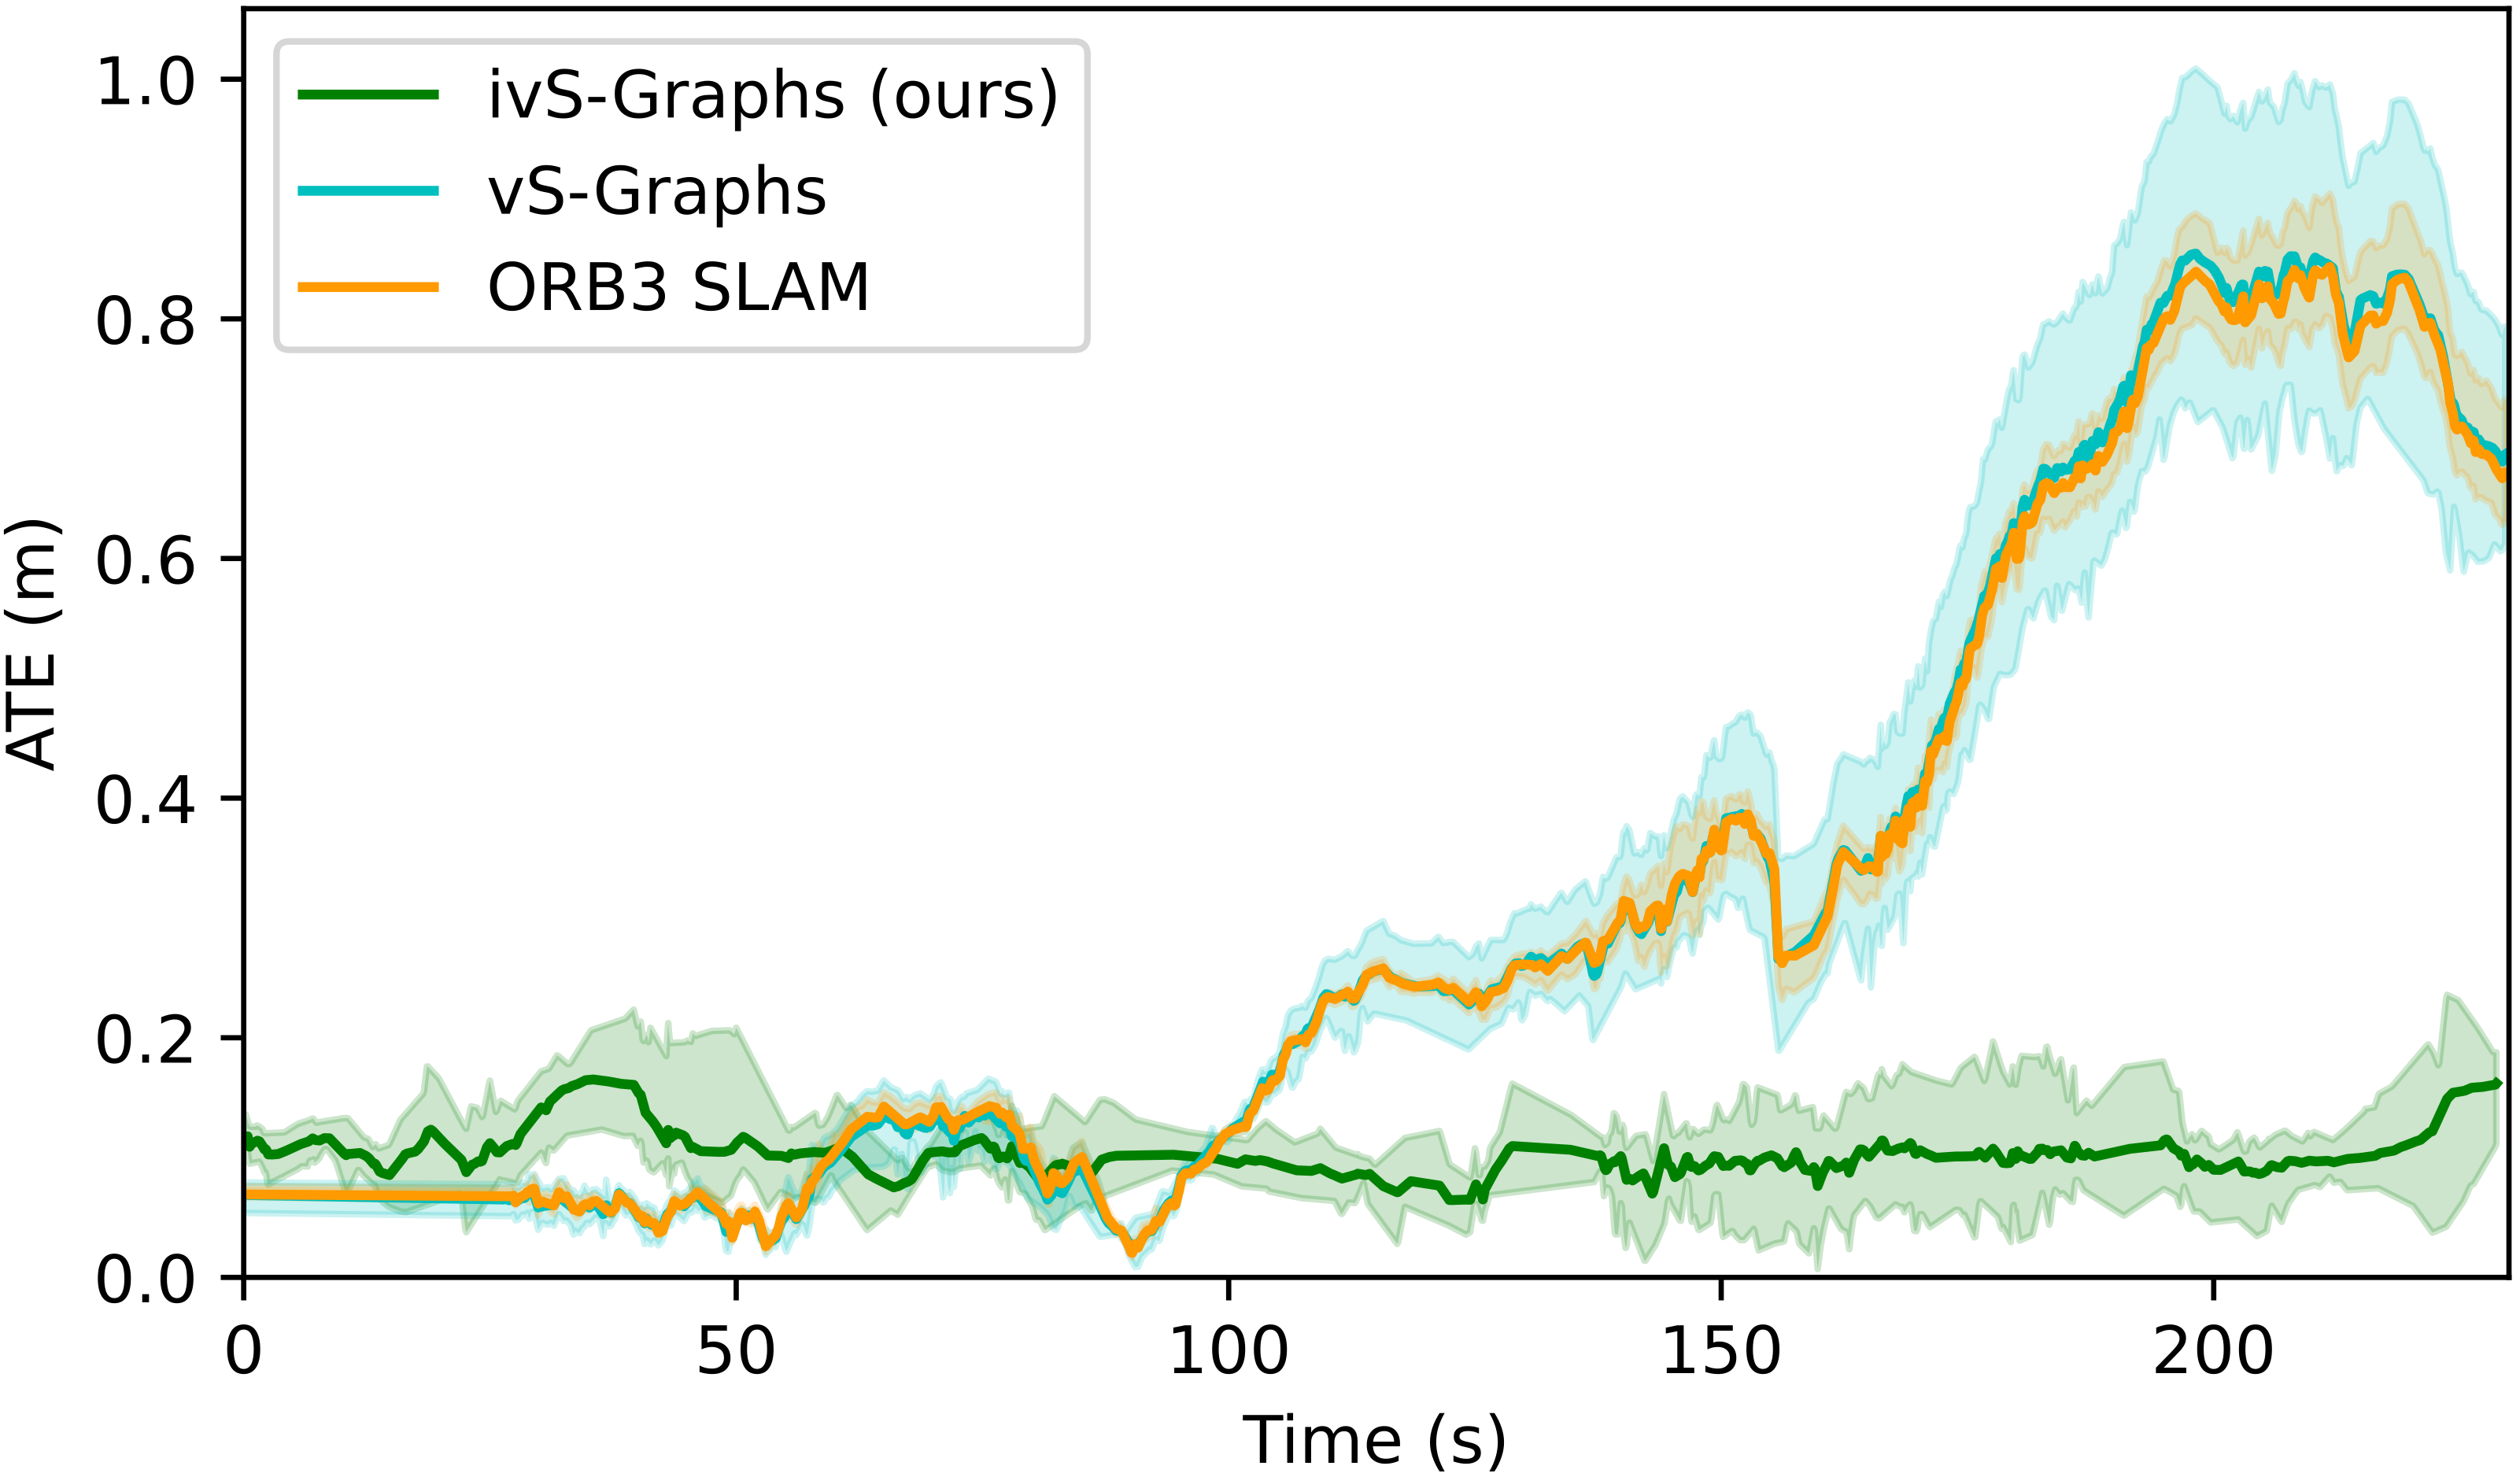
\includegraphics[width=0.4\textwidth]{Figures/Figure_drift.png}
    \caption{Accumulated trajectory drift error over time in \textit{office1-2} sequence, showing the ATE for baselines and \textit{ivS-Graphs}. 
    }
    \label{fig:accumulated_drift}
\end{figure}

The qualitative comparison in Fig.~\ref{fig:qualitative_trajectory} further confirms this trend, showing a top-down overlay of the estimated trajectories on the \textit{office1-1} sequence. For the \textit{vS-Graphs} baseline (right), only the initial semantic alignment is used to display the \textit{as-planned} data. The trajectory estimated by \textit{ivS-Graphs} (left) is topologically consistent with the floor layout, whereas \textit{vS-Graphs} exhibits deviations, with the trajectory crossing through BIM walls. 
The remaining baselines also struggled: BAD-SLAM~\cite{badslam} failed to track in 6 out of 11 sequences due to textureless surfaces, while DROID-SLAM~\cite{droidslam} remained more robust but still exhibited significant drift.


\begin{figure}[b!]
    \centering
    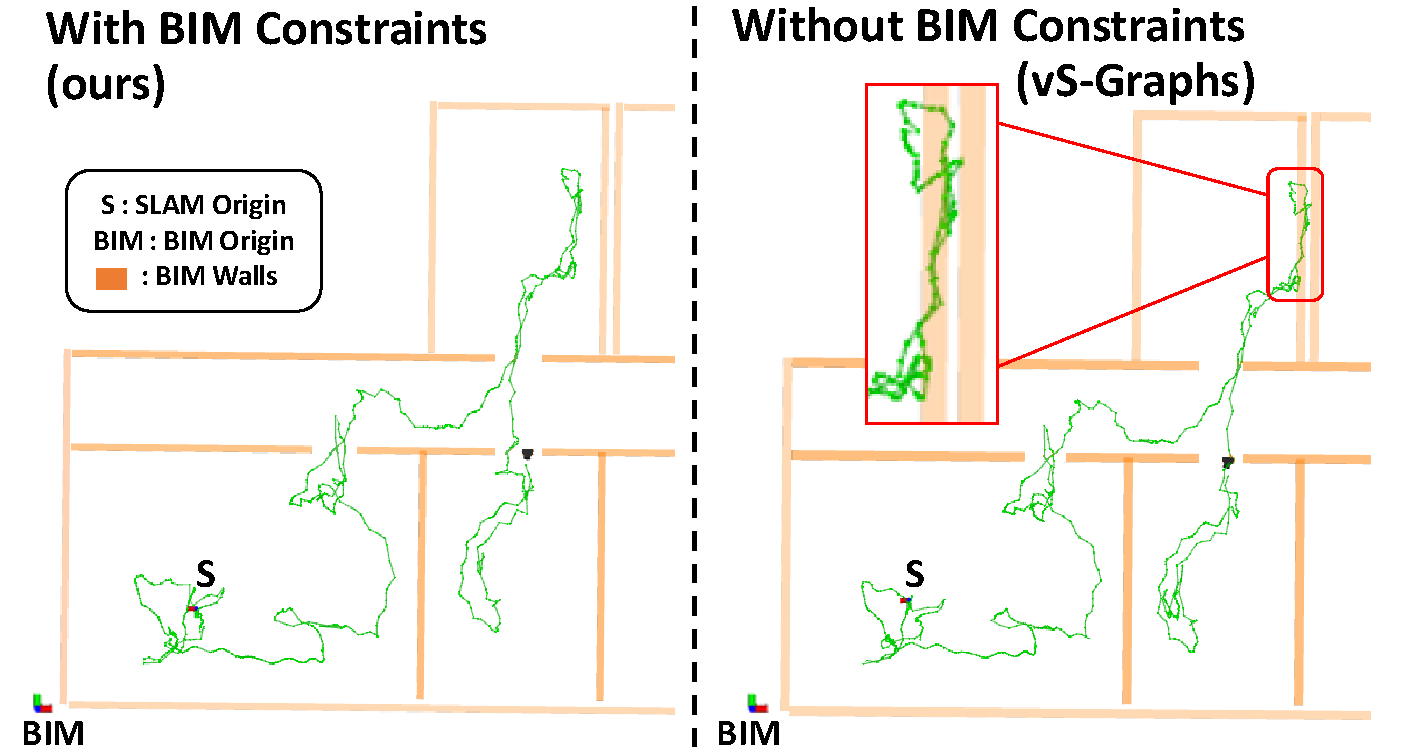
\includegraphics[width=\linewidth]{Figures/qualitative.pdf}
    % \caption{Qualitative comparison of estimated trajectories on the \textit{office1-1} sequence. Left: proposed method with BIM constraints; right: baseline without BIM constraints, just initial alignment integrated.}
    \caption{Top-down overlay trajectory overlay on \textit{office1-1}. Left: \textit{ivS-Graphs} (with BIM). Right: \textit{vS-Graphs} (init. align. only)}
    \label{fig:qualitative_trajectory}
\end{figure}


\add{\subsubsection{\textbf{Wall-Matching Precision}}
Table~\ref{tbl_eval} reports the wall-matching precision per sequence, achieving a mean of 92.8\%. Most mismatches occur between coplanar walls from adjacent rooms. Since the back-end optimization uses only the planar component $\pi = (\mathbf{n}, d)$ of each wall, coplanar walls produce identical constraints and the mismatch does not affect trajectory accuracy. The single true mismatch in \textit{office2-3} is successfully down-weighted by the Huber kernel, as confirmed by its competitive ATE of $0.176\,\text{m}$.}


\subsubsection{\textbf{Mapping Performance}}  
Table~\ref{tbl_RMSE} summarizes the mapping accuracy results. 
\textit{ivS-Graphs} achieves lower point cloud RMSE than the \textit{vS-Graphs} backbone in 9 out of 11 sequences, with improvements on those sequences ranging from +0.99\% to +17.88\%.
The gains follow a clear size-dependent pattern: in larger environments such as \textit{office1-1} (+17.88\%) and \textit{CS1} (+9.63\%), where trajectory drift accumulates over extended operation, BIM constraints produce consistent and meaningful map improvements. In smaller environments, where the baseline trajectory is already accurate, the contribution of BIM integration is marginal. This also explains why the relative gains are smaller than those observed for ATE: BIM constraints reduce drift-induced map distortion but cannot compensate for the per-frame depth noise of the RGB-D sensor, which remains an independent source of map error.


\begin{table}[t!]
 \vspace{0.25cm}
    \centering
    \footnotesize
    \setlength{\tabcolsep}{2.2pt}
    \caption{Root Mean Square Error (RMSE) in meters of reconstructed point clouds for the evaluated \acs{VSLAM} algorithms. The best and second-best results are \textbf{boldfaced} and \underline{underlined}, respectively. Values are averaged over 5 runs. The minimum completion rate of each sequence is set to 50\%, and dashes indicate missing data due to tracking failure. The final column reports the improvement of \textit{ivS-Graphs} over \textit{vS-Graphs}.
    }
    
    \resizebox{\columnwidth}{!}{
    \begin{tabular}{l|ccccc|c}
        \toprule
            \multirow{4}{*}{{\textbf{Sequence}}} & \multicolumn{6}{c}{\textbf{Point Cloud RMSE ($\mathrm{m}$)}} \\
        \cmidrule{2-7}
            & {\shortstack{\textit{BAD} \\ \textit{SLAM} \\ \cite{badslam}}} 
            & {\shortstack{\textit{ORB-} \\ \textit{SLAM 3} \\ \cite{orb3}}} 
            & {\shortstack{\textit{DROID-} \\ \textit{SLAM} \\ \cite{droidslam}}} 
            & {\shortstack{\textit{\vgraphs} \\ \cite{tourani2025vsgraphs}}} 
            & {\shortstack{\textit{\ivgraphs}\\(ours)}} 
            & \textit{Diff. (\%)} \\
        \midrule
           office1-1  & -     & 0.416 & 0.430 & \underline{0.403} & \textbf{0.331} & {+17.88\%} \\
           office1-2  & 0.442 & 0.537 & \underline{0.435} & 0.444 & \textbf{0.396} & {+10.72\%} \\
           office1-3  & -     & 0.360 & 0.395 & \textbf{0.340} & \underline{0.354} & {-4.15\%} \\
           office1-4  & -     & 0.349 & \underline{0.323} & 0.327 & \textbf{0.306} & {+6.35\%} \\
         \midrule
            office2-1 & 0.394 & 0.407 & \textbf{0.371} & 0.432 & \underline{0.382} & {+11.55\%} \\
            office2-2 & -     & 0.487 & \textbf{0.404} & \underline{0.470} & 0.473 & {-0.80\%} \\
            office2-3 & -     & \underline{0.412} & 0.466 & 0.481 & \textbf{0.411} & {+14.60\%} \\
            office2-4 & -     & \textbf{0.386} & \underline{0.460} & 0.546 & 0.504 & {+7.64\%} \\
        \midrule
            CS1       & 0.299 & 0.282 & \textbf{0.252} & 0.307 & \underline{0.277} & {+9.63\%} \\
        \midrule
            CS2-Mid & \textbf{0.357} & 0.425 & 0.268 & 0.378 & \underline{0.374} & {+0.99\%} \\
        \midrule
            CS3-Furn  & -     & 0.588 & \underline{0.296} & 0.298 & \textbf{0.287} & {+3.62\%} \\
        \midrule
             \textbf{Mean} & - & 0.422 & \underline{0.373} & 0.402 & \textbf{0.371} & \multicolumn{1}{c}{{+7.14\%}} \\
        \bottomrule
    \end{tabular}
    }
    \label{tbl_RMSE}
\end{table}


\begin{table}[b]
    \centering
    \caption{ATE [m] under varying BIM completeness. Nominal uses the full model; 20\% and 30\% Miss. omit walls. Rel. Err. shows ATE increase from Nominal to 30\% Missing case.}
    \label{tab:ate_missing_walls}
    \begin{tabular}{l|c|c|c|c}
    \toprule
    \textbf{Sequence} & \textbf{Nominal} & \textbf{20\% Miss.} & \textbf{30\% Miss.} & \textbf{Rel. Err. (\%)} \\
    \midrule
    office1-1 & 0.226 & 0.244 & 0.253 & +11.9\% \\
    CS1 & 0.100 & 0.104 & 0.094 & -6.0\% \\
    CS2-Mid & 0.156 & 0.188 & 0.166 & +6.4\% \\
    CS3-Furn & 0.149 & 0.157 & 0.162 & +8.7\% \\
    \midrule
    \textbf{Mean} & \textbf{0.158} & \textbf{0.173} & \textbf{0.169} & \textbf{+5.3\%} \\
    \bottomrule
    \end{tabular}
\end{table}

\subsubsection{\textbf{Robustness to Model Incompleteness and Deviations}} 
Table~\ref{tab:ate_missing_walls} demonstrates the ATE results for robustness in partially constructed environments. With 30\% of walls missing, the system experiences only 5.3\% average error increase. This minimal degradation occurs because missing walls reduce structural constraints without introducing erroneous information; the remaining 70\% continue to provide drift correction.


\begin{table}[t]
    \centering
     \vspace{0.25cm}
     % \caption{\addtwo{ATE [m] and Match Rate (MR \%) under geometric deviations, reported as ATE / MR. Moderate ($\pm 0.2\,\text{m}$, $\pm 5^\circ$) and Severe ($\pm 0.8\,\text{m}$, $\pm 15^\circ$) perturbations are applied to the BIM walls. Rel. Err. indicates ATE \% increase over Nominal, whose MR is 100\% for all sequences. Moderate and Severe values are averaged over 5 randomized runs, with $\pm$ the standard deviation.}}
     \caption{\addtwo{ATE [m] and Match Rate (MR \%) under geometric deviations, reported as ATE / MR. Moderate ($\pm 0.2\,\text{m}$, $\pm 5^\circ$) and Severe ($\pm 0.8\,\text{m}$, $\pm 15^\circ$) perturbations, averaged over 5 randomized runs ($\pm$ standard deviation), are applied to the BIM walls. Rel. Err. indicates ATE \% increase over Nominal, whose MR is 100\% for all sequences.}}
    \label{tab:deviations}
    \footnotesize
    \resizebox{\columnwidth}{!}{%
    \addtwo{%
    \begin{tabular}{l | c | c | c | cc}
    \toprule
    \multirow{2}{*}{\textbf{Seq.}} & \textbf{Nom.} & \textbf{Moderate} & \textbf{Severe} & \multicolumn{2}{c}{\textbf{Rel. Err. (\%)}} \\
    & ATE & ATE / MR & ATE / MR & \textbf{Mod.} & \textbf{Sev.} \\
    \midrule
    off1-1      & 0.23 & 0.29\,{\scriptsize$\pm$0.05}\,/\,96.0\,{\scriptsize$\pm$5.5} & 0.30\,{\scriptsize$\pm$0.16}\,/\,78.0\,{\scriptsize$\pm$8.4} & +28.3 & +33.4 \\
    CS1         & 0.10 & 0.16\,{\scriptsize$\pm$0.06}\,/\,91.3\,{\scriptsize$\pm$9.5} & 0.16\,{\scriptsize$\pm$0.04}\,/\,85.0\,{\scriptsize$\pm$12.2} & +63.4 & +64.1 \\
    CS2-Mid     & 0.16 & 0.18\,{\scriptsize$\pm$0.04}\,/\,80.0\,{\scriptsize$\pm$13.9} & 0.22\,{\scriptsize$\pm$0.09}\,/\,73.3\,{\scriptsize$\pm$22.4} & +12.5 & +38.0 \\
    CS3-Furn    & 0.15 & 0.18\,{\scriptsize$\pm$0.08}\,/\,94.5\,{\scriptsize$\pm$5.0} & 0.40\,{\scriptsize$\pm$0.26}\,/\,81.8\,{\scriptsize$\pm$6.4} & +20.2 & +167.7 \\
    \midrule
    \textbf{Mean} & \textbf{0.16} & \textbf{0.20 / 90.4} & \textbf{0.27 / 79.5} & \textbf{+28.0} & \textbf{+71.1} \\
    \bottomrule
    \end{tabular}%
    }%
    }
\end{table}

Table~\ref{tab:deviations} evaluates the system's robustness by quantifying the impact of geometric discrepancies on localization accuracy (ATE) and wall association (MR). \addtwo{In every run, initialization succeeded within $\tau_{init}$, keeping the \textit{as-planned} and \textit{as-built} models close enough for the subsequent wall matching to progressively reduce their misalignment.} In the Moderate scenario, which applies realistic construction tolerances to all walls simultaneously, the Match Rate remains high (\changetwo{88.0}{90.4}\%) because deviations fall within association thresholds as they can be misinterpreted as accumulated drift. The back-end optimization incorporates these deviated constraints, resulting in \changetwo{25.8}{28.0}\% average error increase, with the Huber kernel down-weighting the largest residuals preventing catastrophic failure.

The Severe scenario reveals two distinct failure modes. When MR remains high (e.g., CS3-Furn: \changetwo{90.9}{81.8}\% MR), highly deviated walls continue to match and mislead the optimization, causing \changetwo{143.6}{167.7}\% error increase. Conversely, when large deviations trigger rejection (e.g., \changetwo{office1-1: 64.7}{CS2-Mid: 73.3}\% MR), the system relies more on visual baseline, with a lower \changetwo{40.7}{38.0}\% error increase.
This demonstrates that rejecting ambiguous associations outperforms accepting incorrect matches, and that even under deviations far exceeding typical construction tolerances, the system degrades predictably.

\begin{table}[b]
    \centering
    \caption{Runtime performance. FPS is the average processing rate over the trajectory. Align. is the one-time initial registration cost. Match and Opt. (ms) are the mean per-call costs of continuous wall matching (per detected wall) and BIM back-end optimization.}
    \label{tab:runtime}
    \setlength{\tabcolsep}{3pt}
    \begin{tabular}{l|c|ccccc}
    \toprule
    \multirow{2}{*}{\textbf{Sequence}} & \textbf{vS-Graphs} & \multicolumn{5}{c}{\textbf{ivS-Graphs (Ours)}} \\
    \cmidrule(lr){3-7}
    & \textbf{FPS [6]} & \textbf{FPS} & \shortstack{\textbf{Align.}\\\textbf{(ms)}} & \shortstack{\textbf{Match}\\\textbf{(ms)}} & \shortstack{\textbf{Opt.}\\\textbf{(ms)}} & \shortstack{\textbf{Opt.}\\\textbf{calls}} \\
    \midrule
    office1-1   & 23.8 & 21.8 & 0.24 & 0.06 & 843 & 67 \\
    CS1         & 23.3 & 22.5 & 0.23 & 0.07 & 542 & 38 \\
    CS2-Mid     & 24.2 & 23.9 & 0.34 & 0.06 & 321 & 22 \\
    CS3-Furn    & 25.5 & 24.9 & 0.15 & 0.05 & 442 & 18 \\
    \midrule
    \textbf{Mean} & \textbf{24.2} & \textbf{23.3} & \textbf{0.24} & \textbf{0.06} & \textbf{542} & \textbf{36} \\
    \bottomrule
    \end{tabular}
\end{table}


\subsubsection{\textbf{Runtime analysis}} 
Finally, we report a runtime analysis in Table~\ref{tab:runtime} to confirm that the system operates in real time. Across all experiments, \textit{ivS-Graphs} consistently maintained processing rates between 21.8 and 24.9\,FPS (averaging 23.3\,FPS), staying above the 20\,FPS real-time threshold. While this is lower than the 29.3\,FPS average achieved by \textit{ORB-SLAM3}~\cite{orb3}, the difference is primarily due to the additional computational cost of the \textit{Scene Segmentor} and the subsequent structural element extraction. 
\add{The \textit{Match} and \textit{Opt.} columns of Table~\ref{tab:runtime} isolate the BIM-specific cost.
\addtwo{Match performs an unindexed linear scan over the BIM wall database, giving $O(N)$ complexity, but its cost (0.07\,ms, our highest measured cost) is negligible when compared with Opt.'s cost ($\sim$540\,ms average), several orders of magnitude larger.} \changetwo{Opt.'s per-call cost is dominated by newly added associations and the number of poses being corrected; established associations contribute little, as their residuals have already converged.}{Opt.'s per-call cost is driven by trajectory length rather than wall count: office1-1, the longest of these four sequences, has the highest cost despite fewer walls than CS1 or CS2-Mid.} 
\addtwo{Neither cost affects the system's real-time frame rate reported above, since Match and Opt. run in the local mapping thread, decoupled from tracking. For substantially larger buildings, more complex optimization strategies may become necessary. Hierarchical strategies, such as per-room or per-floor optimization~\cite{bavle2025s}, could be implemented, but this is out of the scope of this work.}}
Additionally, the initial alignment is performed in only 0.24\,ms,
which is negligible for system startup.


\subsubsection{\textbf{Limitations}}
\addtwo{Wall detection is bounded by the depth-sensing range of the RGB-D camera feeding the \textit{Scene Segmentor}, which extracts the detected walls $\mathbf{W_S}$ only within this range, with accuracy degrading near the limit. The sensor should therefore be selected according to the depth range required by the target environment.}
\addtwo{These same detection limits bear directly on initialization: if the two intended walls go undetected (occluded, out of range, or otherwise not mapped) or the operator specifies the wrong wall IDs, the acceptance checks ($\tau_\perp$, $\tau_{init}$, Table~\ref{tab:parameters}) are not satisfied, initialization does not occur, and the system runs as the SLAM backbone. If a wrong pair coincidentally satisfies these checks, the resulting alignment is wrong, producing unexpected results.}